\subsection{Формула Тейлора}
Пусть функция \( n \) раз дифференцируема. \\
Рассмотрим формулу дифференцируемой функции:
\[ f(x) = f(x_0) + f'(x_0)(x-x_0) + o(x-x_0) \]
Рассмотрим бесконечно малую функцию \( o(x-x_0) \):
\[ o(x-x_0) = c_2(x-x_0)^2 + o_2(x-x_0), c_2 \in \R \]
%% Добавить иллюстрацию 1 - images/1.jpg (jpg -> tikz)
\begin{figure} 
    \centering
    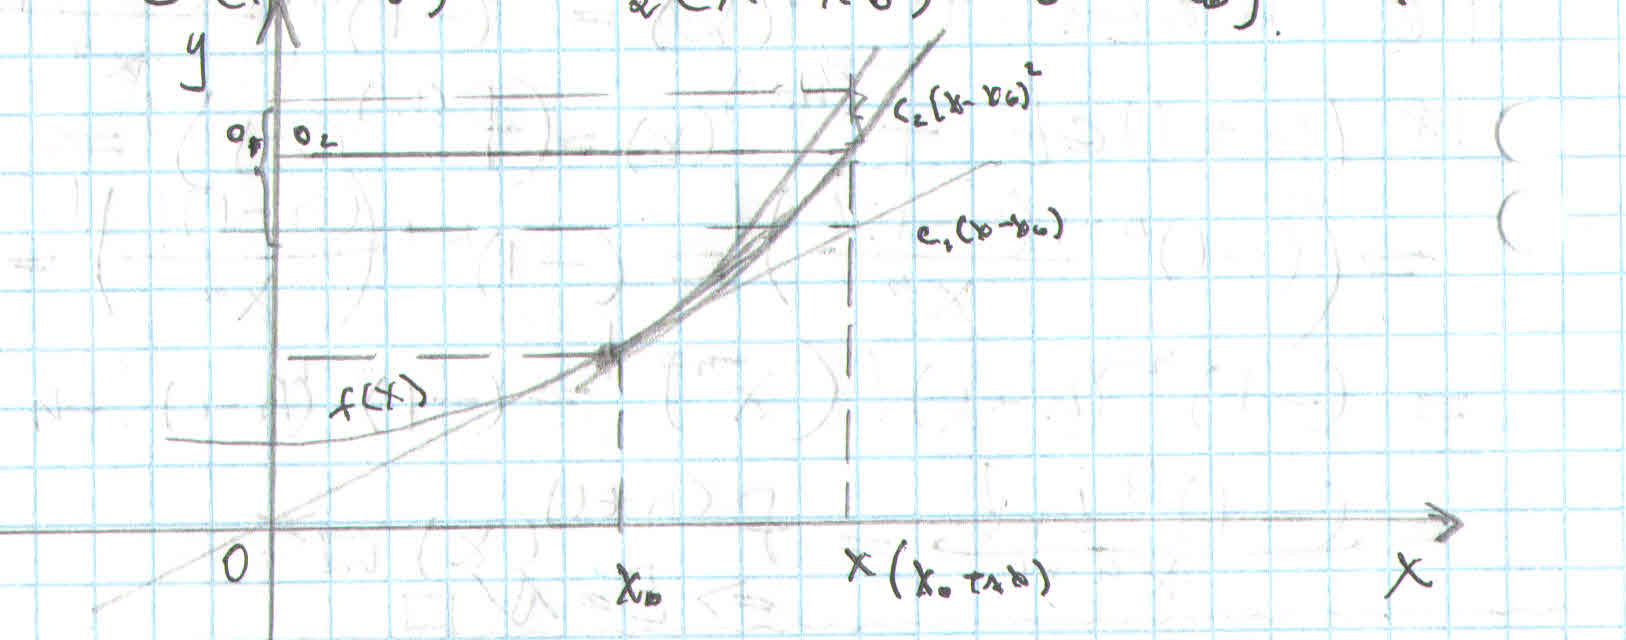
\includegraphics[width=0.5\textwidth]{1}
    \caption{\label{fig:diffGeom} Приближение при помощи дифференциалов}
\end{figure} \\ 
Продолжая так раскрывать все последующие бесконечно малые, мы получим следующую картину:
\[ f(x) = c_1(x-x_0)+c_2(x-x_0)^2+\dots+c_n(x-x_0)^n+R_n(x) \]
Остаётся узнать, какие коэффициенты \( c_{1}, \dots, c_{n} \) нужно подставить. \\ 
\[ c_k = \frac{f^{(k)}(x_0)}{k!} \text{-- коэффициенты Тейлора} \]
Пусть \( P(x) \) -- полином: 
\[ P(x) = \mum{i=1}{n}{c_i(x-x_0)^i} \]
Тогда \( R_n(x) \)(остаток Тейлора) будет равен \( 0 \).
\[ P(x_0) = f(x_0) \]
\[ P'(x_0) = c_1 \Longrightarrow c_1 = \frac{P'(x_0)}{1!} \]
\[ P''(x_0) = 2c_2 \Longrightarrow c_2 = \frac{P''(x_0)}{2!} \]
\[ P'''(x_0) = 6c_3 \Longrightarrow c_3 = \frac{P'''(x_0)}{3!} \]
Таким образом, \[ c_k = \frac{P^{(k)}(x_0)}{k!} \]
Рассмотрим функцию \( f \). Коэффициенты будем строить так же: \( c_k  = \frac{f^{(k)}(x_0)}{k!}\) -- построим полином \( T_n \) (многочлен Тейлора) для \( n \) раз дифференцируемой функции:
\[ T_n(x) = \mum{k=0}{n}{\frac{f^{(k)}(x_0)}{k!}(x-x_0)^k} \]
Но \( T_n \) и \( f \) в общем случае не совпадают - нам нужно добавить \( R_n \) -- остаточный член формулы Тейлора (остаток формулы Тейлора).
\begin{note} 
    При \(x_0 = 0\) коэффициенты, многочлен и формула носят имя Маклорена:
    \begin{itemize} 
        \item \( c_k  = \frac{f^{(k)}(x_0)}{k!} \) - коэффициент Маклорена;
        \item \( T_n(x) = \mum{k=0}{n}{\frac{f^{(k)}(x_0)}{k!}x^k} \) - многочлен Маклорена;
        \item \( f(x) = \mum{k=0}{n}{\frac{f^{(k)}(x_0)}{k!}x^k + R_n(x)}\) - формула Маклорена с остатком;
    \end{itemize}
    % Cлегка неказисто, однако именно так, я полагаю, предполагал лектор в пособии (Да, именно формула с остатком, так как читатель
    % еще не выяснил на данный момент, что остаток данной формулы будет равен нулю при условии, что \(f^{n}\) определена в окрестности 0)
\end{note}